% Options for packages loaded elsewhere
\PassOptionsToPackage{unicode}{hyperref}
\PassOptionsToPackage{hyphens}{url}
%
\documentclass[
  ignorenonframetext,
]{beamer}
\title{R crash course: A quick introduction to R}
\author{Alex Sanchez, Miriam Mota, Ricardo Gonzalo and\\
Santiago Perez-Hoyos}
\date{Statistics and Bioinformatics Unit. Vall d'Hebron Institut de
Recerca}

\usepackage{pgfpages}
\setbeamertemplate{caption}[numbered]
\setbeamertemplate{caption label separator}{: }
\setbeamercolor{caption name}{fg=normal text.fg}
\beamertemplatenavigationsymbolsempty
% Prevent slide breaks in the middle of a paragraph
\widowpenalties 1 10000
\raggedbottom
\setbeamertemplate{part page}{
  \centering
  \begin{beamercolorbox}[sep=16pt,center]{part title}
    \usebeamerfont{part title}\insertpart\par
  \end{beamercolorbox}
}
\setbeamertemplate{section page}{
  \centering
  \begin{beamercolorbox}[sep=12pt,center]{part title}
    \usebeamerfont{section title}\insertsection\par
  \end{beamercolorbox}
}
\setbeamertemplate{subsection page}{
  \centering
  \begin{beamercolorbox}[sep=8pt,center]{part title}
    \usebeamerfont{subsection title}\insertsubsection\par
  \end{beamercolorbox}
}
\AtBeginPart{
  \frame{\partpage}
}
\AtBeginSection{
  \ifbibliography
  \else
    \frame{\sectionpage}
  \fi
}
\AtBeginSubsection{
  \frame{\subsectionpage}
}
\usepackage{amsmath,amssymb}
\usepackage{lmodern}
\usepackage{iftex}
\ifPDFTeX
  \usepackage[T1]{fontenc}
  \usepackage[utf8]{inputenc}
  \usepackage{textcomp} % provide euro and other symbols
\else % if luatex or xetex
  \usepackage{unicode-math}
  \defaultfontfeatures{Scale=MatchLowercase}
  \defaultfontfeatures[\rmfamily]{Ligatures=TeX,Scale=1}
\fi
\usetheme[]{Copenhagen}
\usecolortheme{dolphin}
\usefonttheme{structurebold}
% Use upquote if available, for straight quotes in verbatim environments
\IfFileExists{upquote.sty}{\usepackage{upquote}}{}
\IfFileExists{microtype.sty}{% use microtype if available
  \usepackage[]{microtype}
  \UseMicrotypeSet[protrusion]{basicmath} % disable protrusion for tt fonts
}{}
\makeatletter
\@ifundefined{KOMAClassName}{% if non-KOMA class
  \IfFileExists{parskip.sty}{%
    \usepackage{parskip}
  }{% else
    \setlength{\parindent}{0pt}
    \setlength{\parskip}{6pt plus 2pt minus 1pt}}
}{% if KOMA class
  \KOMAoptions{parskip=half}}
\makeatother
\usepackage{xcolor}
\IfFileExists{xurl.sty}{\usepackage{xurl}}{} % add URL line breaks if available
\IfFileExists{bookmark.sty}{\usepackage{bookmark}}{\usepackage{hyperref}}
\hypersetup{
  pdftitle={R crash course: A quick introduction to R},
  pdfauthor={Alex Sanchez, Miriam Mota, Ricardo Gonzalo and Santiago Perez-Hoyos},
  hidelinks,
  pdfcreator={LaTeX via pandoc}}
\urlstyle{same} % disable monospaced font for URLs
\newif\ifbibliography
\usepackage{color}
\usepackage{fancyvrb}
\newcommand{\VerbBar}{|}
\newcommand{\VERB}{\Verb[commandchars=\\\{\}]}
\DefineVerbatimEnvironment{Highlighting}{Verbatim}{commandchars=\\\{\}}
% Add ',fontsize=\small' for more characters per line
\usepackage{framed}
\definecolor{shadecolor}{RGB}{248,248,248}
\newenvironment{Shaded}{\begin{snugshade}}{\end{snugshade}}
\newcommand{\AlertTok}[1]{\textcolor[rgb]{0.94,0.16,0.16}{#1}}
\newcommand{\AnnotationTok}[1]{\textcolor[rgb]{0.56,0.35,0.01}{\textbf{\textit{#1}}}}
\newcommand{\AttributeTok}[1]{\textcolor[rgb]{0.77,0.63,0.00}{#1}}
\newcommand{\BaseNTok}[1]{\textcolor[rgb]{0.00,0.00,0.81}{#1}}
\newcommand{\BuiltInTok}[1]{#1}
\newcommand{\CharTok}[1]{\textcolor[rgb]{0.31,0.60,0.02}{#1}}
\newcommand{\CommentTok}[1]{\textcolor[rgb]{0.56,0.35,0.01}{\textit{#1}}}
\newcommand{\CommentVarTok}[1]{\textcolor[rgb]{0.56,0.35,0.01}{\textbf{\textit{#1}}}}
\newcommand{\ConstantTok}[1]{\textcolor[rgb]{0.00,0.00,0.00}{#1}}
\newcommand{\ControlFlowTok}[1]{\textcolor[rgb]{0.13,0.29,0.53}{\textbf{#1}}}
\newcommand{\DataTypeTok}[1]{\textcolor[rgb]{0.13,0.29,0.53}{#1}}
\newcommand{\DecValTok}[1]{\textcolor[rgb]{0.00,0.00,0.81}{#1}}
\newcommand{\DocumentationTok}[1]{\textcolor[rgb]{0.56,0.35,0.01}{\textbf{\textit{#1}}}}
\newcommand{\ErrorTok}[1]{\textcolor[rgb]{0.64,0.00,0.00}{\textbf{#1}}}
\newcommand{\ExtensionTok}[1]{#1}
\newcommand{\FloatTok}[1]{\textcolor[rgb]{0.00,0.00,0.81}{#1}}
\newcommand{\FunctionTok}[1]{\textcolor[rgb]{0.00,0.00,0.00}{#1}}
\newcommand{\ImportTok}[1]{#1}
\newcommand{\InformationTok}[1]{\textcolor[rgb]{0.56,0.35,0.01}{\textbf{\textit{#1}}}}
\newcommand{\KeywordTok}[1]{\textcolor[rgb]{0.13,0.29,0.53}{\textbf{#1}}}
\newcommand{\NormalTok}[1]{#1}
\newcommand{\OperatorTok}[1]{\textcolor[rgb]{0.81,0.36,0.00}{\textbf{#1}}}
\newcommand{\OtherTok}[1]{\textcolor[rgb]{0.56,0.35,0.01}{#1}}
\newcommand{\PreprocessorTok}[1]{\textcolor[rgb]{0.56,0.35,0.01}{\textit{#1}}}
\newcommand{\RegionMarkerTok}[1]{#1}
\newcommand{\SpecialCharTok}[1]{\textcolor[rgb]{0.00,0.00,0.00}{#1}}
\newcommand{\SpecialStringTok}[1]{\textcolor[rgb]{0.31,0.60,0.02}{#1}}
\newcommand{\StringTok}[1]{\textcolor[rgb]{0.31,0.60,0.02}{#1}}
\newcommand{\VariableTok}[1]{\textcolor[rgb]{0.00,0.00,0.00}{#1}}
\newcommand{\VerbatimStringTok}[1]{\textcolor[rgb]{0.31,0.60,0.02}{#1}}
\newcommand{\WarningTok}[1]{\textcolor[rgb]{0.56,0.35,0.01}{\textbf{\textit{#1}}}}
\setlength{\emergencystretch}{3em} % prevent overfull lines
\providecommand{\tightlist}{%
  \setlength{\itemsep}{0pt}\setlength{\parskip}{0pt}}
\setcounter{secnumdepth}{-\maxdimen} % remove section numbering
\ifLuaTeX
  \usepackage{selnolig}  % disable illegal ligatures
\fi

\begin{document}
\frame{\titlepage}

\begin{frame}{Readme}
\protect\hypertarget{readme}{}
\begin{itemize}
\item
  License: Creative Commons Attribution-NonCommercial-ShareAlike 4.0
  International License
  \url{http://creativecommons.org/licenses/by-nc-sa/4.0/}
\item
  You are free to:

  \begin{itemize}
  \tightlist
  \item
    \textbf{Share} : copy and redistribute the material
  \item
    \textbf{Adapt} : rebuild and transform the material
  \end{itemize}
\item
  Under the following conditions:

  \begin{itemize}
  \tightlist
  \item
    \textbf{Attribution} : You must give appropriate credit, provide a
    link to the license, and indicate if changes were made.
  \item
    \textbf{NonCommercial} : You may not use this work for commercial
    purposes.
  \item
    \textbf{Share Alike} : If you remix, transform, or build upon this
    work, you must distribute your contributions under the same license
    to this one.
  \end{itemize}
\end{itemize}
\end{frame}

\hypertarget{a-crash-course-in-r}{%
\section{A Crash Course in R}\label{a-crash-course-in-r}}

\begin{frame}{Outline}
\protect\hypertarget{outline}{}
\begin{itemize}
\tightlist
\item
  Why R

  \begin{itemize}
  \tightlist
  \item
    R basics
  \item
    How does one work with R and Rstudio
  \end{itemize}
\item
  Getting Started

  \begin{itemize}
  \tightlist
  \item
    A primer of data import
  \item
    Variables and data types
  \item
    Functions, Packages and more stuff
  \end{itemize}
\item
  Working with data

  \begin{itemize}
  \tightlist
  \item
    \emph{Selecting, Filtering and ordering datasets}
  \item
    \emph{A primer of statistics and plots}
  \item
    R Notebooks and RMarkdown
  \end{itemize}
\end{itemize}
\end{frame}

\begin{frame}{Motivation}
\protect\hypertarget{motivation}{}
\begin{itemize}
\item
  We (you) all work with data, most of the time and often we need to do
  ``things'' with those data.

  \begin{itemize}
  \tightlist
  \item
    I have three lists of genes and I would like to see which genes they
    have in common (or which ones appear only in one list).
  \item
    We have received the data from that lab but I only want to work with
    a subset of the samples.
  \item
    Is it possible to repeat that plot changing the line colors, the
    font size etc?
  \item
    I have some scripts tu re-run an analysis but I don't know how to
    start
  \end{itemize}
\item
  These, and many other things can be done with a basic knowledge of R.
\end{itemize}
\end{frame}

\begin{frame}{\href{https://www.r-project.org/about.html}{What is R?}}
\protect\hypertarget{what-is-r}{}
\begin{itemize}
\item
  R is a \emph{language and environment} for statistical computing and
  graphics.
\item
  R provides a wide variety of statistical and graphical techniques, and
  is highly extensible.
\item
  It can be used fro simple tasks to highly complex reproducible
  projects.
\item
  It compiles and runs on a wide variety of UNIX platforms and similar
  systems Windows and MacOS.
\end{itemize}
\end{frame}

\begin{frame}{How is R used}
\protect\hypertarget{how-is-r-used}{}
\begin{itemize}
\tightlist
\item
  Different ways to use R, but the best trade-off simplicity-efficiency
  is provided by Rstudio
\end{itemize}

\begin{figure}
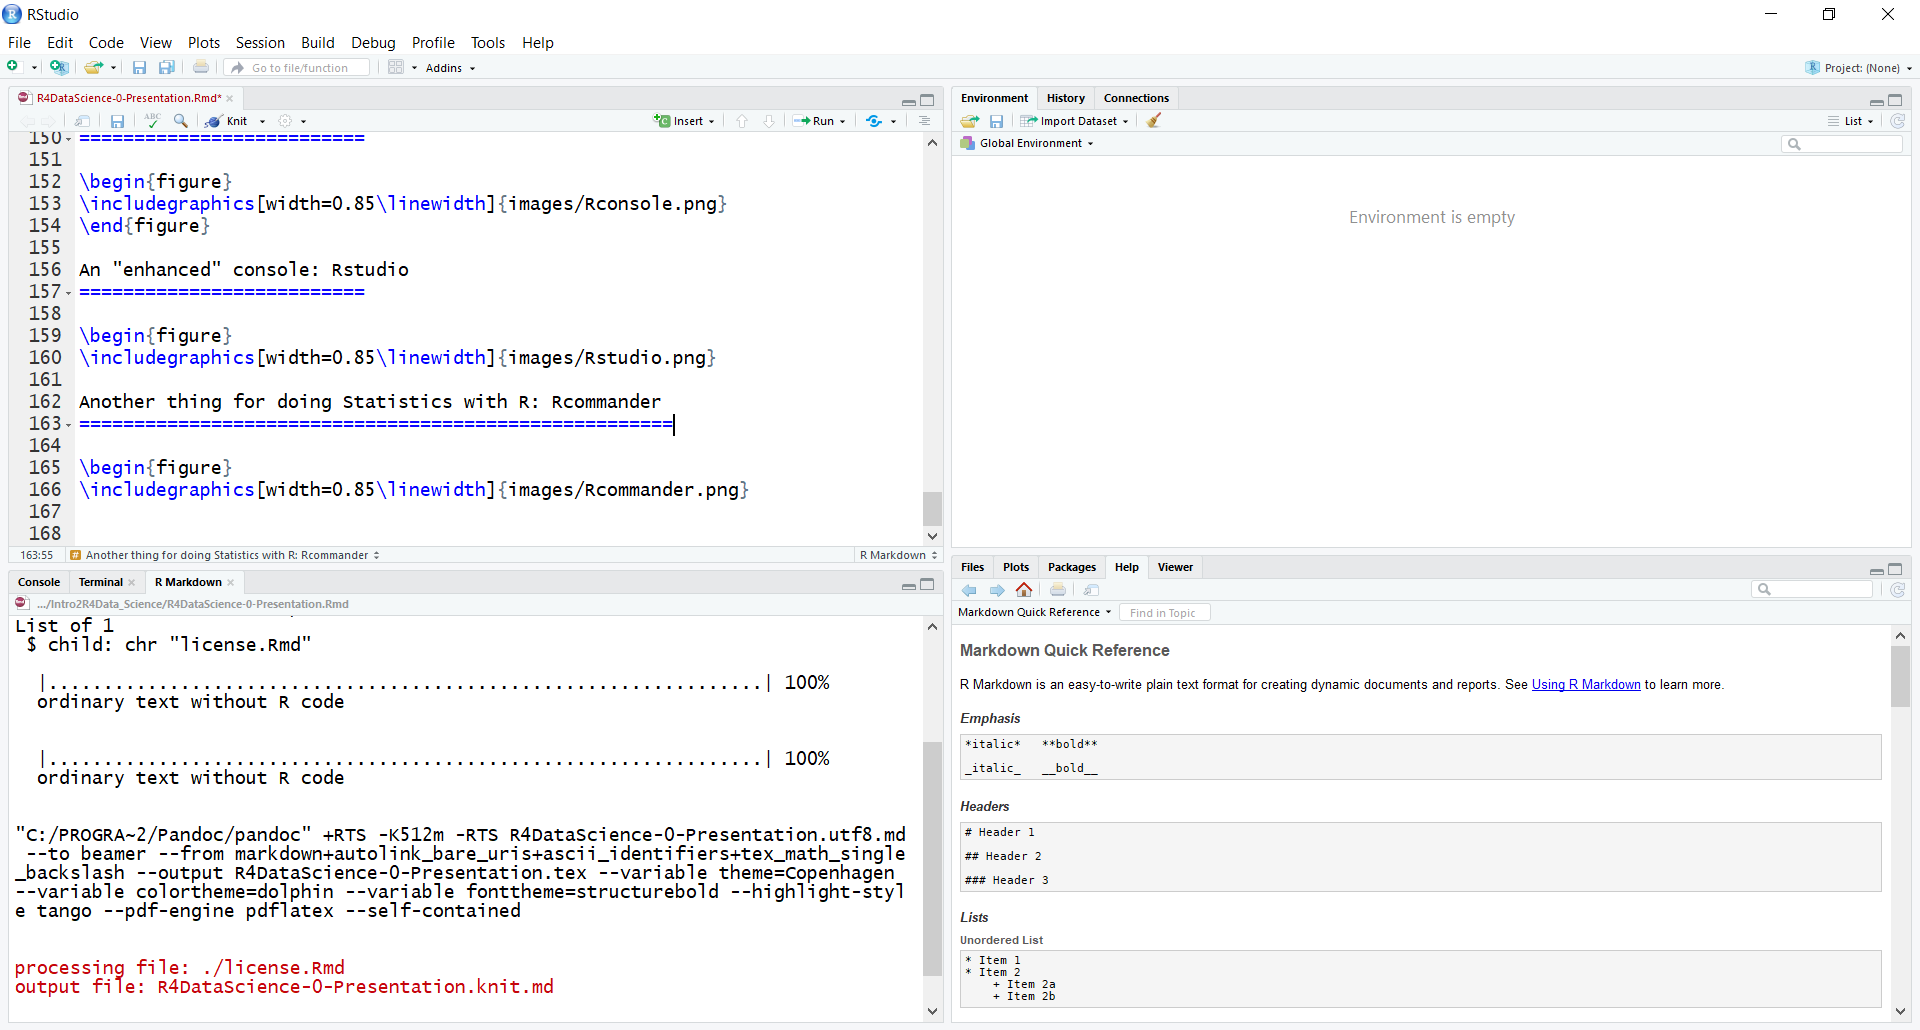
\includegraphics[width=0.85\linewidth]{images/RStudio.png}
\end{figure}
\end{frame}

\begin{frame}{Exercise}
\protect\hypertarget{exercise}{}
\begin{itemize}
\item
  Get to know R. Visit the R-project page and see what can be found
  there.
\item
  If you haven't done it before, download and install R and Rstudio in
  your computer
\item
  Open R studio. Look at the panels and figgure out what can we do at
  each window.
\end{itemize}
\end{frame}

\hypertarget{using-r}{%
\section{Using R}\label{using-r}}

\begin{frame}{Commands, Objects and Functions}
\protect\hypertarget{commands-objects-and-functions}{}
\begin{itemize}
\tightlist
\item
  Shortly, using R consists of

  \begin{itemize}
  \tightlist
  \item
    Working with \emph{objects} using \emph{commands} and
    \emph{functions}
  \end{itemize}
\end{itemize}

\begin{figure}
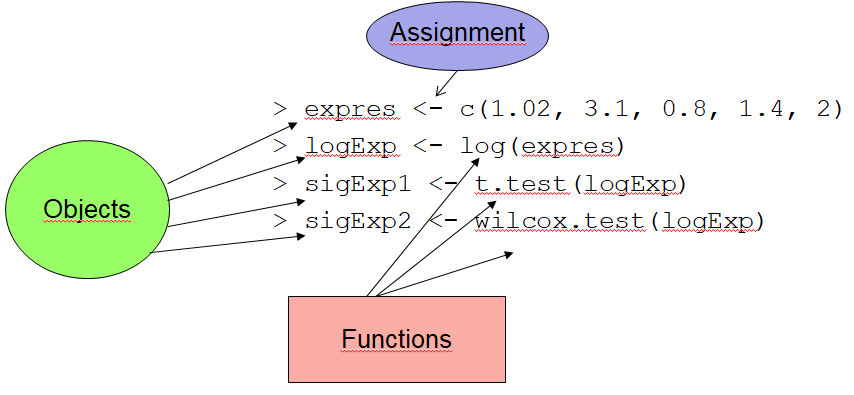
\includegraphics[width=0.85\linewidth]{images/basicConcepts.png}
\end{figure}
\end{frame}

\begin{frame}{Variables and data types}
\protect\hypertarget{variables-and-data-types}{}
\begin{itemize}
\tightlist
\item
  Data managed in R \ldots{}

  \begin{itemize}
  \tightlist
  \item
    is stored as \emph{variables}
  \end{itemize}
\item
  Variables can be of distinct types

  \begin{itemize}
  \tightlist
  \item
    Numerical

    \begin{itemize}
    \tightlist
    \item
      numeric (13.7)
    \item
      int (3)
    \end{itemize}
  \item
    Character

    \begin{itemize}
    \tightlist
    \item
      ``R is cute''
    \end{itemize}
  \item
    Factors

    \begin{itemize}
    \tightlist
    \item
      A,B,C,D
    \item
      WT, Mut
    \end{itemize}
  \end{itemize}
\end{itemize}
\end{frame}

\begin{frame}{R packages}
\protect\hypertarget{r-packages}{}
\begin{itemize}
\tightlist
\item
  R can be used for many different types of data processing and analysis
  from distinct fields, besides statistics such as Ecology, Omics
  Sciences, Psychology etc.
\item
  All these capabilities are not present from the begining because most
  of them will never be used by most users.
\item
  Instead, thay can be added when needed by

  \begin{enumerate}
  [(i)]
  \tightlist
  \item
    installing and
  \item
    loading the appropriate packages.
  \end{enumerate}
\end{itemize}
\end{frame}

\begin{frame}[fragile]{Installing and loading packages}
\protect\hypertarget{installing-and-loading-packages}{}
We want to analyze some data using cox proportional hazards model.

\begin{Shaded}
\begin{Highlighting}[]
\NormalTok{res.cox }\OtherTok{\textless{}{-}} \FunctionTok{coxph}\NormalTok{(}\FunctionTok{Surv}\NormalTok{(time, status) }\SpecialCharTok{\textasciitilde{}}\NormalTok{ sex, }\AttributeTok{data =}\NormalTok{ lung)}
\end{Highlighting}
\end{Shaded}

\texttt{Error\ in\ coxph(Surv(time,\ status)\ \textasciitilde{}\ sex,\ data\ =\ lung)\ :\ could\ not\ find\ function\ "coxph"}

We need to install and load the package before we can use it.

\begin{Shaded}
\begin{Highlighting}[]
\FunctionTok{install.packages}\NormalTok{(}\StringTok{"survival"}\NormalTok{)}
\FunctionTok{library}\NormalTok{(survival)}
\NormalTok{res.cox }\OtherTok{\textless{}{-}} \FunctionTok{coxph}\NormalTok{(}\FunctionTok{Surv}\NormalTok{(time, status) }\SpecialCharTok{\textasciitilde{}}\NormalTok{ sex, }\AttributeTok{data =}\NormalTok{ lung)}
\end{Highlighting}
\end{Shaded}
\end{frame}

\begin{frame}{Bioconductor}
\protect\hypertarget{bioconductor}{}
\begin{itemize}
\tightlist
\item
  Packages analyse all kinds of Genomic data (\textgreater800)
\item
  Compulsory documentation (\emph{vignettes}) for each package
\item
  6-month release cycle
\item
  \href{http://bioconductor.org/help/course-materials/}{Course
  Materials}
\item
  \href{http://bioconductor.org/packages/release/BiocViews.html\#___ExperimentData}{Example
  data} and \href{http://bioconductor.org/help/workflows/}{workflows}
\item
  Common, re-usable framework and functionality
\item
  \href{https://support.bioconductor.org/}{Available Support}

  \begin{itemize}
  \tightlist
  \item
    Often you will be able to interact with the package maintainers /
    developers and other power-users of the project software
  \end{itemize}
\end{itemize}
\end{frame}

\begin{frame}[fragile]{The \texttt{tidyverse}}
\protect\hypertarget{the-tidyverse}{}
\begin{itemize}
\tightlist
\item
  The tidyverse is an opinionated collection of R packages designed for
  data science.
\item
  All packages share an underlying design philosophy, grammar, and data
  structures.
\item
  The complete tidyverse collection can be installed with:
\end{itemize}

\begin{Shaded}
\begin{Highlighting}[]
\FunctionTok{install.packages}\NormalTok{(}\StringTok{"tidyverse"}\NormalTok{)}
\end{Highlighting}
\end{Shaded}

\begin{itemize}
\tightlist
\item
  \url{https://www.tidyverse.org/}
\end{itemize}
\end{frame}

\hypertarget{getting-data-into-r}{%
\section{Getting data into R}\label{getting-data-into-r}}

\begin{frame}[fragile]{Importing data with Rstudio}
\protect\hypertarget{importing-data-with-rstudio}{}
\begin{itemize}
\tightlist
\item
  The easiest way to get data into R is to click on the
  \texttt{Ìmport\ Datasets} button.
\item
  Alternatively R code can be written using functions from
  \texttt{Base\ R} or the \texttt{tidyverse}

  \begin{itemize}
  \tightlist
  \item
    \texttt{Base\ R} functions start with \texttt{read.}:
    \texttt{read.table}, \texttt{read.csv}
  \item
    \texttt{tidyverse} functions start with \texttt{read\_}:
    \texttt{read\_delim}, \texttt{read\_csv} or \texttt{read\_excel}
  \end{itemize}
\end{itemize}
\end{frame}

\begin{frame}{Reading Excel or csv files}
\protect\hypertarget{reading-excel-or-csv-files}{}
\begin{itemize}
\tightlist
\item
  Files can be read from any location, let it be a physical support or a
  web site.
\item
  To read files from disk be sure to indicate their location.
\item
  Alternatively the default working directory can be set to the folder
  where the file is located.
\end{itemize}
\end{frame}

\begin{frame}[fragile]{Reading Excel or csv files (continued)}
\protect\hypertarget{reading-excel-or-csv-files-continued}{}
\begin{itemize}
\item
  Assume files \texttt{TIO2+PTYR-human-MSS+MSIvsPD.XLSX} has been
  downloaded to your working directory
\item
  Start setting the default directory to the folder where you have saved
  the file.

  \begin{itemize}
  \tightlist
  \item
    \texttt{Session\ -\/-\textgreater{}\ Set\ Working\ directory\ -\/-\textgreater{}\ To\ source\ file\ location...}
  \end{itemize}
\item
  Import the \texttt{TIO2+PTYR-human-MSS+MSIvsPD.XLSX} with the default
  options
\end{itemize}
\end{frame}

\begin{frame}[fragile]{Reading Excel or csv files (continued)}
\protect\hypertarget{reading-excel-or-csv-files-continued-1}{}
\begin{Shaded}
\begin{Highlighting}[]
\CommentTok{\# Read Excel file}
\FunctionTok{library}\NormalTok{(readxl)}
\NormalTok{otherData }\OtherTok{\textless{}{-}} \FunctionTok{read\_excel}\NormalTok{(}\StringTok{"otherFiles"}\NormalTok{)}
\end{Highlighting}
\end{Shaded}

\begin{itemize}
\tightlist
\item
  Code generated for reading the files can be reused any time changing
  the file name if needed.
\end{itemize}
\end{frame}

\begin{frame}[fragile]{Interlude: Summarizing data}
\protect\hypertarget{interlude-summarizing-data}{}
\begin{itemize}
\tightlist
\item
  Once a dataset is available it is easy to ``have a look at it''
\end{itemize}

\begin{Shaded}
\begin{Highlighting}[]
\FunctionTok{head}\NormalTok{(phosphoprotData)}
\FunctionTok{str}\NormalTok{(phosphoprotData)}
\FunctionTok{summary}\NormalTok{ (phosphoprotData)}
\end{Highlighting}
\end{Shaded}
\end{frame}

\hypertarget{dynamic-output-with-rmarkdown}{%
\section{Dynamic output with
Rmarkdown}\label{dynamic-output-with-rmarkdown}}

\begin{frame}{Reproducible research with R notebooks}
\protect\hypertarget{reproducible-research-with-r-notebooks}{}
\begin{itemize}
\tightlist
\item
  R and Rstudio are strongly involved in promoting
  \href{https://en.wikipedia.org/wiki/Reproducibility}{reproducibility}
  and
  \href{https://en.wikipedia.org/wiki/Reproducibility\#Reproducible_research}{reproducible
  research}.
\item
  This is implemented in \textbf{R notebooks}
\item
  A notebook combines

  \begin{itemize}
  \tightlist
  \item
    Natural language text, e.g.~describing what we are doing in our own
    words.
  \item
    R code with the instructions needed to do the data management or the
    analysis.
  \item
    The output of the analysis
  \end{itemize}
\end{itemize}
\end{frame}

\begin{frame}[fragile]{Creating Notebooks}
\protect\hypertarget{creating-notebooks}{}
\begin{itemize}
\tightlist
\item
  A notebook can be created in Rstudio with

  \begin{itemize}
  \tightlist
  \item
    \texttt{File\ -\/-\textgreater{}\ New\ File\ -\/-\textgreater{}\ R\ Notebook}
  \end{itemize}
\item
  The notebook contains example text and code so it is straightforwoard
  to adapt it to your analysis.
\item
  To produce an html file with text, code and output:

  \begin{itemize}
  \tightlist
  \item
    Press the button ``Preview''
  \item
    Or Select ``Knitr to Html''
  \end{itemize}
\end{itemize}
\end{frame}

\hypertarget{resources-and-exercises}{%
\section{Resources and exercises}\label{resources-and-exercises}}

\begin{frame}{Introductory materials}
\protect\hypertarget{introductory-materials}{}
The web is full of all types of materials about R

Below there are a couple of brief introductions:

\begin{itemize}
\item
  \href{https://stats.idre.ucla.edu/r/seminars/short-introduction-to-r/}{A
  short introduction to R}
\item
  \href{https://github.com/saghirb/Getting-Started-in-R}{Getting started
  with R}
\end{itemize}
\end{frame}

\begin{frame}{Exercise}
\protect\hypertarget{exercise-1}{}
\begin{itemize}
\tightlist
\item
  Select a dataset with which you wish to work along the course.
\item
  Read it into R

  \begin{itemize}
  \tightlist
  \item
    How many variables are there in it
  \item
    What are their types
  \end{itemize}
\item
  Try to summarize it briefly
\item
  Create an R notebook to encapsulate all your steps and share it with
  somebody.
\end{itemize}
\end{frame}

\end{document}
